\documentclass{beamer}
\usetheme{boadilla}
%\useoutertheme{split}
\title[Writer identification task]{Master Thesis proposal:\\Approaches for writer identification in \\
handwritten papyri}
\author{Lorenzo Sala}
\date{\today}
\institute{Stochastics and Data Science}
\begin{document}
\begin{frame}[plain]
    \maketitle
\end{frame}
\begin{frame}
	\frametitle{Outline}
	\begin{itemize}
		\item Introduction on machine learning
		\item State of the art
		\item Two particular approaches to the problem
	\end{itemize}
\end{frame}
\begin{frame}[c]
	\frametitle{Introduction}
	\begin{itemize}
		\item Papyri are an exception among ancient written artifacts in terms of preservation
		\item Most papyri went through the antiquity market where they were scattered around and split apart
		\item Identifying the writer over several fragments is beneficial for philology purposes
		\item Many papyri suffer from similar damage or corruption
		\item Non-harmonized approach in conservation
	\end{itemize}
\end{frame}
\begin{frame}
	\frametitle{The problem of classification}
	\begin{itemize}
		\item We may aim to determine that two different written manuscripts have been written by the same person
		\item Simple human examination is often not enough, especially when dealing with compromised artifacts or with extremely scarce corpora\begin{figure}[h]
			\centering
			
\includegraphics[width=0.4\linewidth]{img/question}
			\label{fig:question}
		\end{figure}	
	\end{itemize}
\end{frame}
\begin{frame}
	\frametitle{Classification tasks}
	\begin{itemize}
		\item We need a way to extract information and patterns from data in a statistically significant way so that we can \textbf{classify} them in groups
		\item There are two main branches of classification methods: \textbf{supervised} and \textbf{unsupervised} classification
		\item \textbf{Supervised} classification: \begin{enumerate}
			\item we start from a ``training'' data set where each object is already labelled as belonging to a class;
			\item we use the ``training'' data to learn characteristics about each label;
			\item we use these learnt characteristics to classify unknown data into one of the labels from the ``training'' data.
		\end{enumerate}
		\item \textbf{Unsupervised classification}:
		\begin{enumerate}
			\item we start from an unlabelled data set;
			\item we cluster data together based on their similarity;
			\item we learn characteristics about those clusters.
		\end{enumerate}
	\end{itemize}
\end{frame}
\begin{frame}
	\frametitle{Unsupervised vs supervised classification}
	\begin{figure}
		\centering
		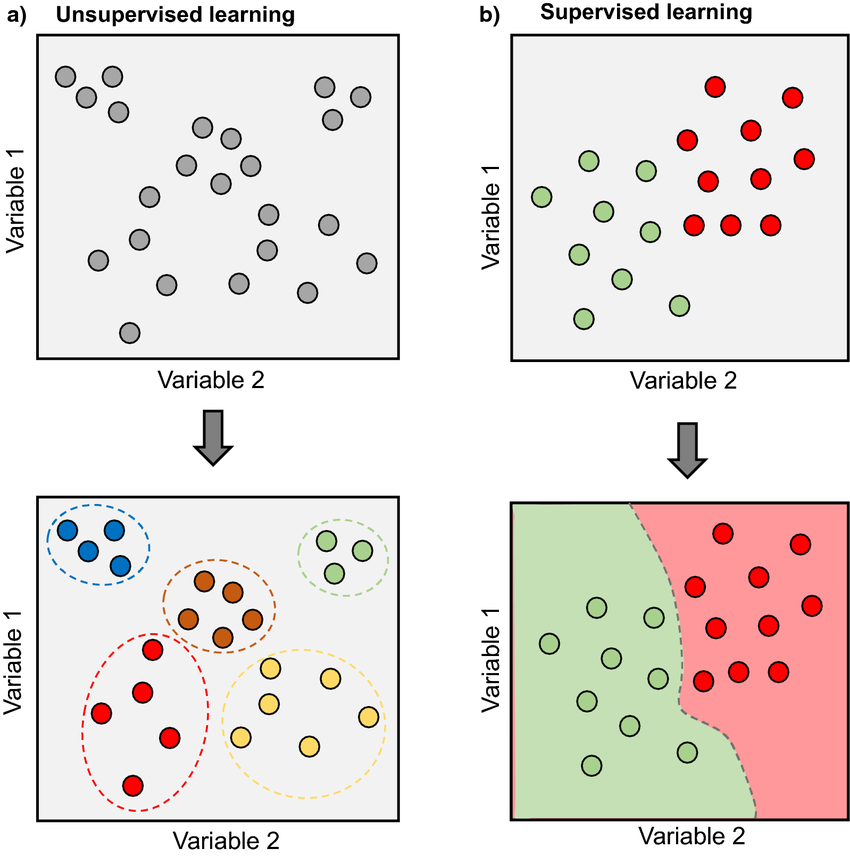
\includegraphics[width=0.5\linewidth]{img/supervised}
		\label{fig:supervised}
	\end{figure}
\end{frame}
\begin{frame}
	\frametitle{Machine learning vs Deep learning}
	\begin{itemize}
		\item Classification tasks broadly fall under the umbrella of Machine Learning
		\item This is a ``classic'' approach, being developed since the 1950s
		\item This approach relies in having a ``machine'' ``learn'' a set of features about data
		\item These features are usually manually extracted or inferred
	\end{itemize}
\end{frame}
\begin{frame}
	\frametitle{Example of machine learning (clustering) algorithms}\begin{figure}[h]
		\centering
		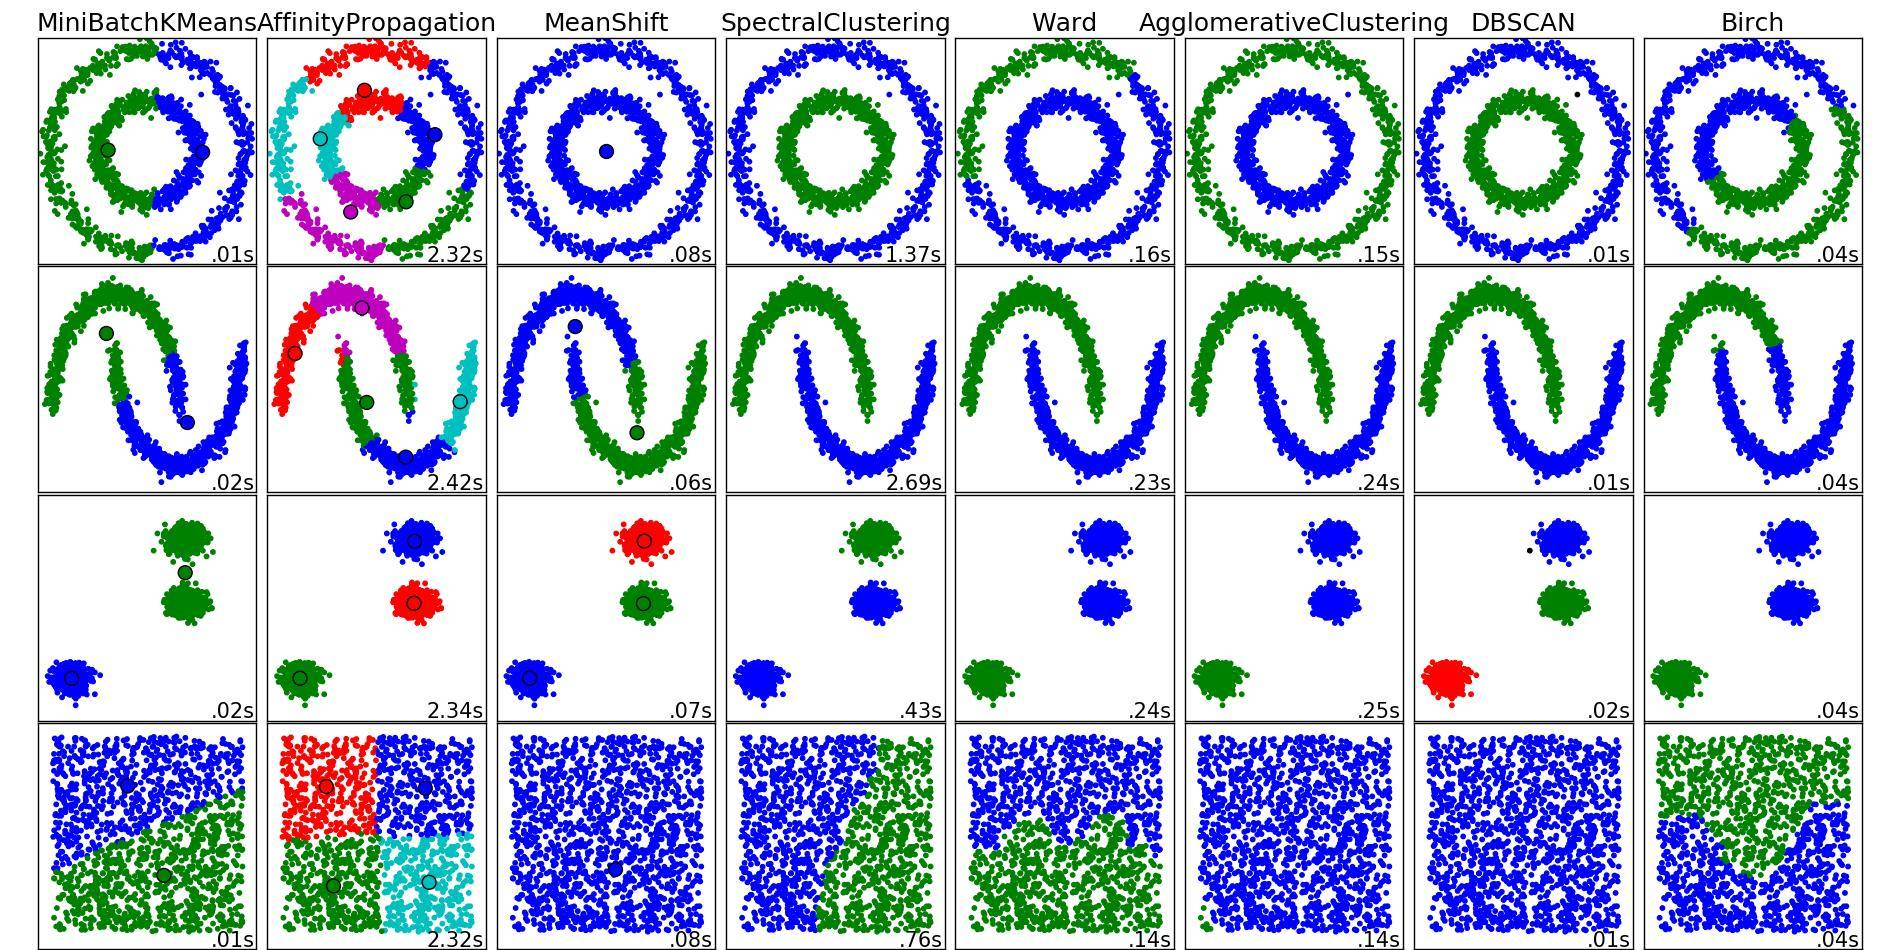
\includegraphics[width=\linewidth]{img/algos}
		\label{fig:algos}
	\end{figure}
\end{frame}
\begin{frame}
	\frametitle{Example of machine learning algorithm (decision trees)}
	\begin{figure}[h]
		\centering
		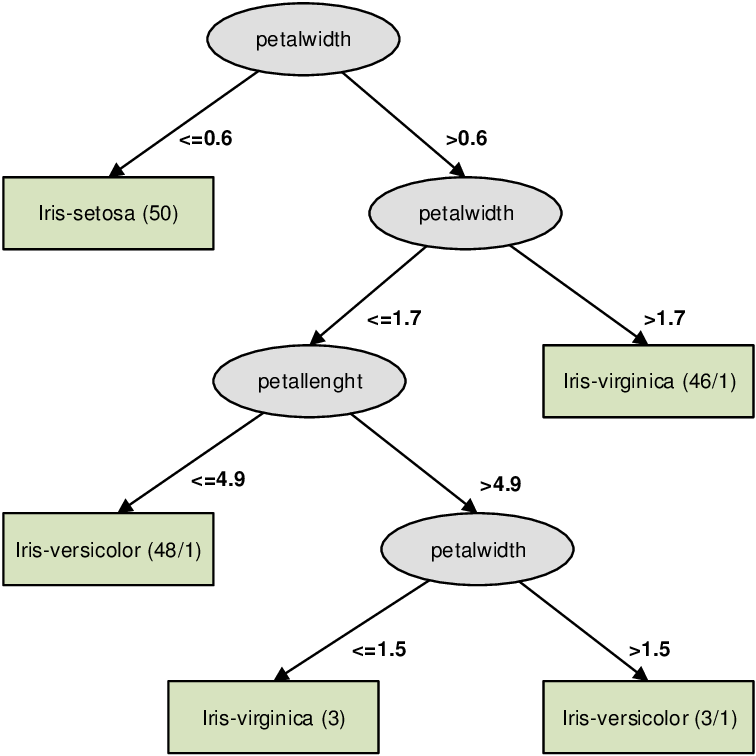
\includegraphics[height=0.7\textheight]{img/decisiontree}
		\label{fig:decisiontree}
	\end{figure}
\end{frame}
\begin{frame}
	\frametitle{Machine learning vs Deep learning}
	\begin{itemize}
		\item In recent years Deep learning approaches have become more and more common
		\item Broadly speaking, they are based on the principle that the algorithm itself should indirectly learn features of the data
		\item This ``learning'' process is pursued by adjusting the internal parameters of a modular network of neurons until the result of the network is not too far from the expected one
		\item Neurons are disposed in layers connected to each other and the stratified structure is what allows the indirect learning
	\end{itemize}
	\begin{figure}[h]
		\centering
		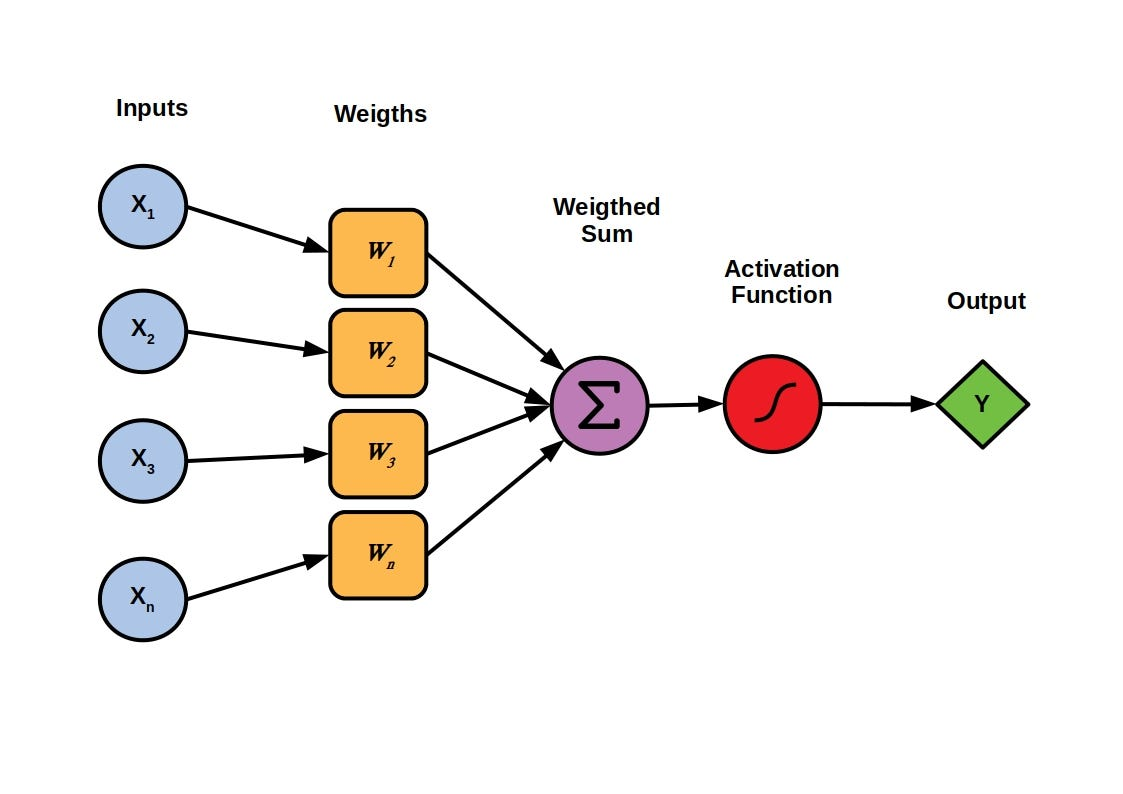
\includegraphics[width=0.5\linewidth]{img/perceptron}
		\label{fig:perceptron}
	\end{figure}
\end{frame}
\begin{frame}
	\frametitle{Convolutional Neural Networks}
	\begin{itemize}
		\item In the field of computer vision, Convolutional Neural Networks have represented a breakthrough
		\item  They are based on a ``convolution kernel'', which can be imagined as a filter that scans the imagine looking for particular features
		\item Instead of being hand-crafted those features are ``learnt'' by the algorithm and then pooled together
	\end{itemize}
	\begin{figure}[h]
		\centering
		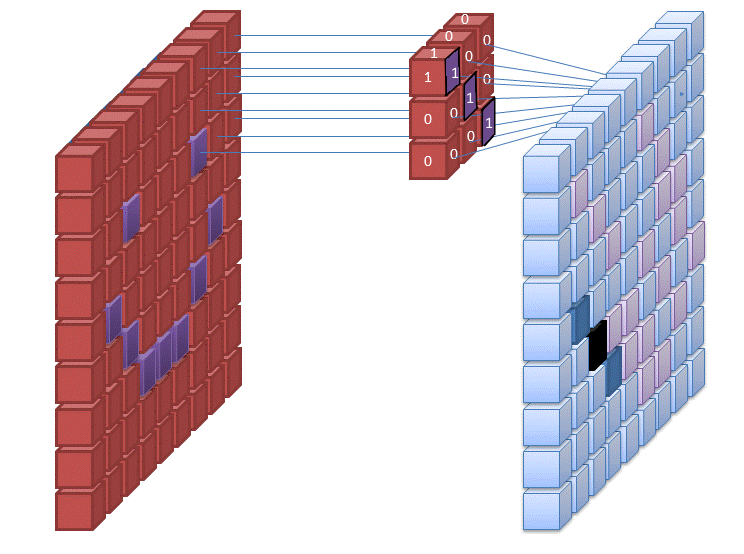
\includegraphics[width=0.5\linewidth]{img/kernel}
		\label{fig:kernel}
	\end{figure}
\end{frame}
\begin{frame}
	\frametitle{Convolutional Neural Networks}
	\begin{itemize}
		\item The process is then repeated so that the CNNs can be seen as a machine learning general visual features starting from small local patterns
	\end{itemize}\begin{figure}[h]
	\centering
	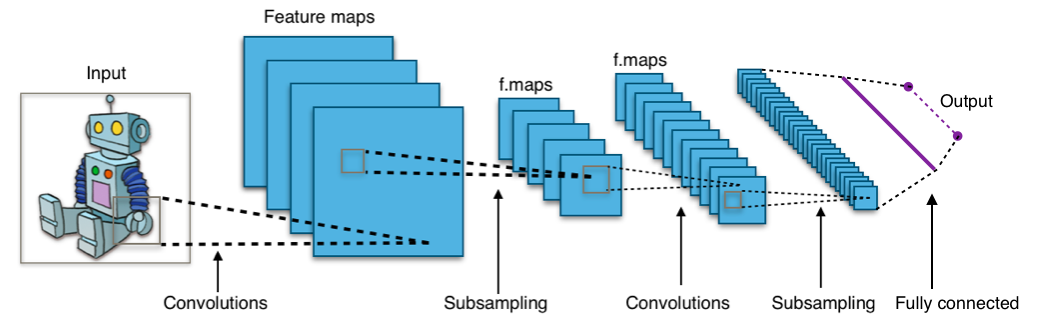
\includegraphics[width=1\linewidth]{img/cnn}
	\label{fig:cnn}
	\end{figure}
\end{frame}
\begin{frame}
	\frametitle{CNNs for writer identification}
	\begin{itemize}
		\item As a staple of computer vision and image classification, CNNs offer an extremely interesting option to learn visual features about handwriting
		\item As such, they are among the preferred methods for classification of handwriting
		\item Those models need a large amount of data needed for training (which is a problem in the case of manuscripts) and a relevant computational effort to run the training and the classification task itself
	\end{itemize}
\end{frame}
\begin{frame}
	\frametitle{A CNN applied to the classification of Greek handwriting (Christlein et al.)}
	\begin{figure}[h]
		\centering
		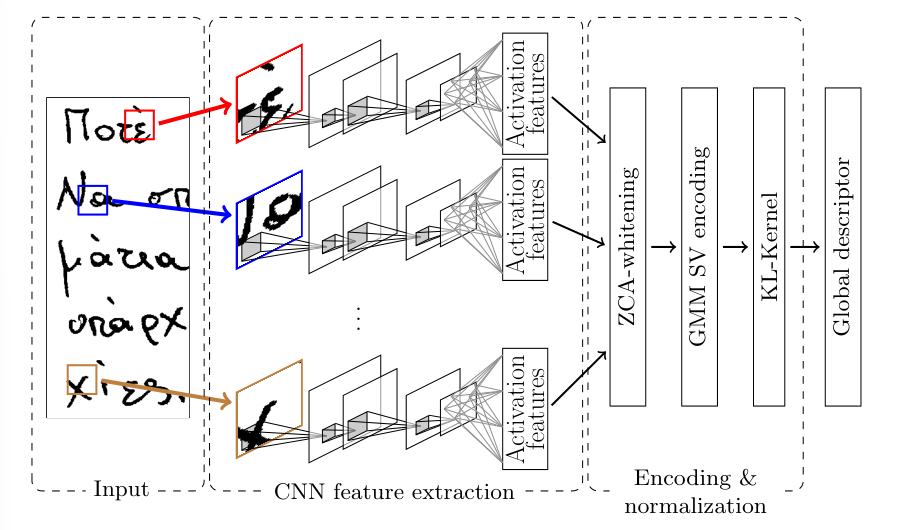
\includegraphics[width=\linewidth]{img/christlein}
		\label{fig:christlein}
	\end{figure}
\end{frame}
\begin{frame}
	\frametitle{Deep learning vs ``classic'' classification tasks}
	\begin{itemize}
		\item Since AlexNet in 2012, CNNs have been widely used in the image recognition field
		\item Nowadays newer techniques like Vision Transformers (e.g. Microsoft's Swim Transformer) offer potential improvements on CNNs
		\item DL techniques allow us:
		\begin{itemize}
			\item to avoid manual feature extraction
			\item to capture finer pattern
			\item to enjoy high flexibility (we can fine-tune models according to different scenarios)
		\end{itemize}
		\item The main drawback lies in the high computational cost and in the need for a significantly large labeled data set
		\item In this particular setting we have an extremely limited number datasets
	\end{itemize}
\end{frame}
\begin{frame}
	\frametitle{State of the art in handwriting identification: non DL approaches}
	\begin{itemize}
		\item Edge-based technique based on the probability density function of orientation and shape usage (Schomaker et al.)
		\item Texture based technique categorizing textures in fragments based on classic LBP/LTP/LPQ analysis. A frequentist analysis is then performed (Hannad et al.)
		\item Texture based technique based on Delta encoding (online, $\Delta x_{t}$ and $\Delta y_{t}$ at each time $t$) and Basic Image Feature Columns (offline, pixel-wise classification) (Hannad et al.)
		\item Quantification of calligraphic style (Zhang et al.)
	\end{itemize}
\end{frame}
\begin{frame}
	\frametitle{State of the art in handwriting identification: non DL approaches}
	\begin{itemize}
		\item Usage of the Levenshtein edit distance based on Fisher-Wagner algorithm to compute the cost of transforming one handwritten word into another (Bensefia et al.)
		\item Usage of computer vision algorithms and statistical inference to identify fragments originated from the same codex (Shweka et al.)
		\item Junction detection method based on ``skeletonization'' of letters to construct the distribution of the direction taken by the letter at each junction, being a global feature for each writer (He et al.)
		\item System based from text layout analysis (De Stefano et al.)
		\item Combining LBP with oriented BIFs column histogram to train a SVM classifier (Abbas et al.)
	\end{itemize}
\end{frame}
\begin{frame}
	\frametitle{State of the art in handwriting identification: DL approaches}
	\begin{itemize}
		\item Residual Swim Transformer: Vision Transformer (CNN which uses attention instead of convolution kernels) with residual connection in ResNet's style (Zhang et al.)
		\item Hybrid approach combining CNNs (for global patterns) with RNNs (for sequential patterns and gine grained information) (GR-RNN)
		\item Identification of keypoints with FAST and Harris detection, creation of small patches centered on keypoints which are fed into a CNN and then using MLE to identify the writer (Semma et al.)
		\item Combining strokes' tickness features with deep features extracted by CNNs (Javidi et al.)
	\end{itemize}
\end{frame}
\begin{frame}
	\frametitle{State of the art in handwriting identification: DL approaches}
	\begin{itemize}
		\item Concatenating deep global features and deep ``restricted'' features computed to obtain graphemes (He et al., Bulacu et al.)
		\item Even stricter restriction of deep features to individual letters and then combining different DL mechanisms (Chen et al.)
		\item RL model guided by human experts that assign idiosyncrasy scores, aimed at detecting excerpts of  maximal idiosyncrasy scores which in turn are used to train a CNN (Adak et al.)
		\item Performing PCA on a diverse set of graphometric features to represent handwriting to train a shallow CNN on a reduced-dimensionality space (Vasquez et al.)
	\end{itemize}
\end{frame}
\begin{frame}
	\frametitle{A possible solution: Christlein's approach}
	\begin{itemize}
		\item Christlein et al. developed a method in 2017 for unsupervised feature learning for writer identification and writer retrieval
		\item In their approach, CNNs are not trained with a supervised approach (since no labeled training set is available)
		\item Instead, they train the CNN in an unsupervised way to extract robust features without determining the identity of the author
	\end{itemize}
\end{frame}
\begin{frame}
	\frametitle{Christlein's approach in writer retrieval}
\begin{itemize}
	\item The main pipeline of the technique is the following:
	\begin{enumerate}
		\item SIFT descriptors are computed on the training dataset
		\item SIFT descriptors are clustered together and clusters become pseudo-labels
		\item Each SIFT keypoint becomes the centre of a patch and a CNN (ResNet) is trained using the cluster membership as target
		\item The activations of the penultimate layer serve as local feature descriptors
		\item Descriptors are encoded and classified
	\end{enumerate}
\end{itemize}
\begin{figure}[h]
	\centering
	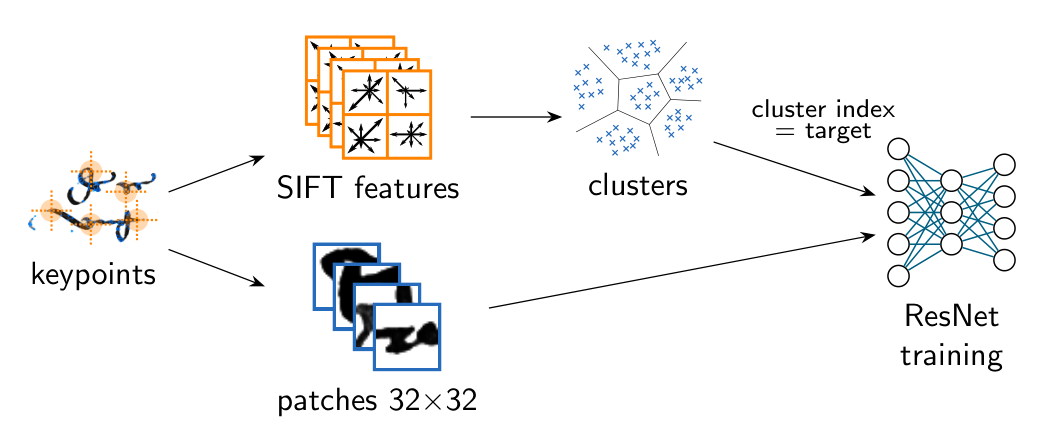
\includegraphics[width=0.7\linewidth]{img/christlein2}
	\label{fig:christlein2}
\end{figure}
\end{frame}
\begin{frame}
	\frametitle{SIFT algorithm}
	\begin{itemize}
	\item 	The Scale Invariant Feature Transform algorithm as been published by David Lowe in 1999. It is free for use since 2020
	\item The basic idea is to extract important points of an object represented in an image so that that object can be recognized in a different image
	\item The SIFT feature descriptor is invariant to uniform scaling, orientation, illumination and partially invariant to distortion
	\item The model is verified by a linear least squares estimation
	\end{itemize} 
	\begin{figure}[h]
		\centering
		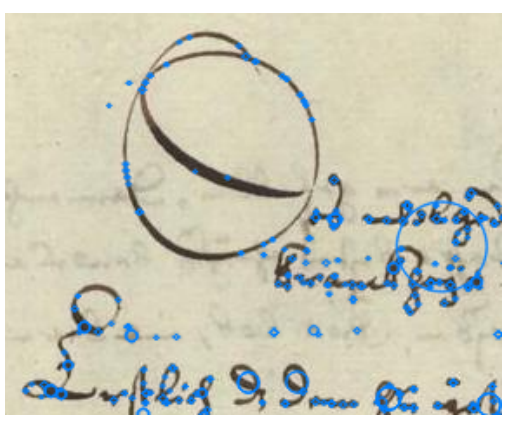
\includegraphics[width=0.3\linewidth]{img/screenshot001}
		\caption{From Christlein's paper: example of (restricted) SIFT keypoints}
		\label{fig:screenshot001}
	\end{figure}
\end{frame}
\begin{frame}
	\frametitle{Clustering and CNN training}
	\begin{itemize}
		\item SIFT descriptors are clustering with a mini-batch version of $k$-means algorithm, filtering out descriptors that lie on the border between two classes
	\item A deep CNN network is trained on the $32\times 32$ image patches and their cluster memberships
	\item The authors use a 20 layers Residual Networks: those are CNNs where the result of a layer is forwarded two layers deeper, skipping the directly following layer. This helps against vanishing gradients and allows for deeper networks.
	\item The results are taken from the penultimal layer which consists in a pooling layer with dimensionality of $64$.
	\item VLAD encoding is used to represent the whole codebook in a single vector
	\item Exemplar SVM are used to classify these global descriptors.
	\end{itemize}
\end{frame}
\begin{frame}
	\frametitle{A possible solution: Mamatsis approach}
	\begin{itemize}
		\item Mamatsis et al. developed a methond in 2023 to establish the authorship of two Greek documents discovered in Romania
		\item Instead of a DL approach, the authors use a geometric approach
		\item This bypasses the inherent problems of CNNs since it doesn't need extensive data for training
		\item It is leagues more computationally efficient
	\end{itemize}
\end{frame}
\begin{frame}
	\frametitle{Mamatsis' approach in writer retrieval}
	The authors propose the following workflow:
		\begin{enumerate}
			\item Bundles of ``optimally fit'' realizations of every alphabet symbol are created
			\item Contours of those bundles are rendered so that they all consists of the same number of pixels
			\item The curvature at the center of each pixel is evaluated via polynomial approximation
			\item A biunivocal correspondence between pixels is realised between pixels with close values of curvature
		\end{enumerate}
\end{frame}
\begin{frame}
	\frametitle{Mamatsis' approach in writer retrieval}
	\begin{enumerate}
		\setcounter{enumi}{4}
		\item Among pixels of common curvature the mean of $x$ and $y$ coordinates is evaluated to obtain an average curved (``First-Version Representative'')
		\item The procedure is repeated in connection with all the First-Version Representatives to form an ``Ideal Representative'' of the form of the alphabet's symbol in the author's mind
		\item For each alphabet symbol separately the Ideal Representatives from two different documents are compared and then a statistical test is used against the hypothesis that the two documents are from the same hand.
	\end{enumerate}
\end{frame}
\begin{frame}
	\frametitle{Steps to find the ideal representative}
	\begin{itemize}
		\item \emph{Optimal matching}: examples of the same symbol are rotated, scaled and translated so that the similarity between them is maximised: this results in a bundle of optimally fit contours
		\item \emph{Suppressing discrepancies}: average curvatures are evaluated and the whole process (including matching) is repeated each time using a different example of a letter as starting prototype. In the end the curve with the least error is chosen
	\end{itemize}
	\begin{figure}[h]
		\centering
		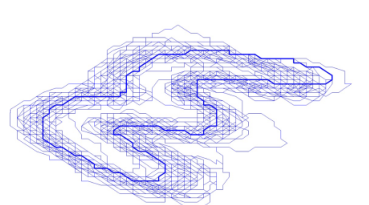
\includegraphics[width=0.4\linewidth]{img/screenshot002}
		\caption{Bundle of optimally fit countours of $\varepsilon$ from Mamatsis' paper}
		\label{fig:screenshot002}
	\end{figure}
\end{frame}
\begin{frame}
	\frametitle{Example of ideal representatives}
	\begin{figure}
		\centering
		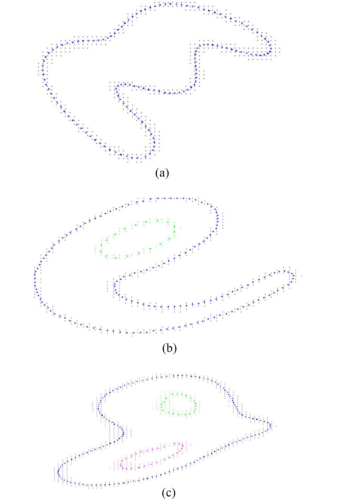
\includegraphics[width=0.4\linewidth]{img/mamatsis1}
		\label{fig:mamatsis1}
	\end{figure}
\end{frame}
\begin{frame}
	\frametitle{Conclusions}
	\begin{itemize}
		\item Different approaches bear different upsides and downsides
		\item Deep Learning approaches are more robust and accurate, but less feasible on a such a limited data pool
		\item Alternative approaches are more easy to realize but may not have the robustness of DL-based techniques
		\item The choose between the two roads is mainly dependent on the particular data available and on computing resources.
	\end{itemize}
\end{frame}
\end{document}
